\documentclass[11pt]{article}
\usepackage[letterpaper,margin=1in]{geometry}
\usepackage[T1]{fontenc}
\usepackage{lmodern,microtype,amsmath,booktabs,graphicx,xcolor,enumitem,multirow}
\usepackage[font=small,labelfont=bf,skip=3pt]{caption}
\usepackage[colorlinks=true,linkcolor=blue!50!black,urlcolor=blue!50!black,citecolor=blue!50!black]{hyperref}
\setlist{nosep,leftmargin=1.2em,topsep=1pt}
\setlength{\parskip}{2.5pt}\setlength{\parindent}{0pt}
\renewcommand{\arraystretch}{1.05}
% generated by note/make_note.py from results/ -- do not edit by hand
\newcommand{\ISsr}{0.98}
\newcommand{\OOSsr}{\ensuremath{-}0.12}
\newcommand{\ISret}{9.0\%}
\newcommand{\OOSret}{3.0\%}
\newcommand{\ISvol}{7.6\%}
\newcommand{\OOSvol}{6.6\%}
\newcommand{\ISdd}{\ensuremath{-}11.7\%}
\newcommand{\OOSdd}{\ensuremath{-}8.7\%}
\newcommand{\ISworst}{\ensuremath{-}4.7\%}
\newcommand{\OOSworst}{\ensuremath{-}2.3\%}
\newcommand{\ISsrtwo}{0.62}
\newcommand{\OOSsrtwo}{\ensuremath{-}0.61}
\newcommand{\ISto}{90}
\newcommand{\OOSto}{108}
\newcommand{\ISgross}{1.35}
\newcommand{\OOSgross}{0.38}
\newcommand{\ISnw}{4.62}
\newcommand{\OOSnw}{\ensuremath{-}0.18}
\newcommand{\ISskew}{1.04}
\newcommand{\ISalpha}{6.2\%}
\newcommand{\ISalphat}{3.95}
\newcommand{\OOSalpha}{\ensuremath{-}1.3\%}
\newcommand{\OOSalphat}{\ensuremath{-}0.35}
\newcommand{\ISbondbeta}{0.31}
\newcommand{\ISmktbeta}{0.05}
\newcommand{\ISmombeta}{0.05}
\newcommand{\bootlo}{0.67}
\newcommand{\boothi}{1.31}
\newcommand{\PBO}{0.023}
\newcommand{\nconfigs}{1,404}
\newcommand{\nsplits}{12,870}
\newcommand{\ntrials}{1,467}
\newcommand{\neff}{3.5}
\newcommand{\DSR}{0.40}
\newcommand{\DSReff}{0.999}
\newcommand{\SRzero}{1.04}
\newcommand{\SRzeroeff}{0.26}
\newcommand{\nbrmed}{0.94}
\newcommand{\bestyr}{11\%}
\newcommand{\cfgmedian}{0.33}
\newcommand{\rollmed}{0.97}
\newcommand{\rollpfive}{0.17}
\newcommand{\rollmin}{\ensuremath{-}0.29}
\newcommand{\rollfrac}{1\%}
\newcommand{\CisIEF}{7.2}
\newcommand{\CoosIEF}{3.0}
\newcommand{\CisOther}{\ensuremath{-}0.4}
\newcommand{\CoosOther}{\ensuremath{-}1.6}
\newcommand{\AisSpr}{11.0}
\newcommand{\AoosSpr}{2.5}
\newcommand{\contA}{\ensuremath{-}1.3\%}
\newcommand{\contC}{\ensuremath{-}0.2\%}
\newcommand{\contT}{1.1\%}
\newcommand{\grossmean}{0.87}
\newcommand{\grossp}{3.88}
\newcommand{\IFCsr}{0.94}
\newcommand{\IFCtwo}{0.61}
\newcommand{\IFCdd}{\ensuremath{-}13.8\%}
\newcommand{\IFCnbr}{0.86}
\newcommand{\IFCalpha}{6.5\%}
\newcommand{\IFCalphat}{3.11}
\newcommand{\IFCdelay}{0.59}
\newcommand{\IFCshiftE}{0.52}
\newcommand{\IFCshiftL}{0.53}
\newcommand{\IFCFsr}{1.05}
\newcommand{\IFCFtwo}{0.92}
\newcommand{\IFCoos}{\ensuremath{-}0.31}
\newcommand{\IFCFoos}{0.01}
\newcommand{\PCTsr}{0.30}
\newcommand{\TSMOMsr}{0.44}
\newcommand{\IDsr}{0.57}
\newcommand{\PCTFsr}{0.24}
\newcommand{\TSMOMFsr}{0.28}
\newcommand{\IDFsr}{0.43}
\newcommand{\PCTFoos}{\ensuremath{-}0.10}
\newcommand{\TSMOMFoos}{0.14}
\newcommand{\IDFoos}{0.06}
\newcommand{\oosA}{\ensuremath{-}0.73}
\newcommand{\oostwoA}{\ensuremath{-}1.01}
\newcommand{\oosB}{\ensuremath{-}0.27}
\newcommand{\oostwoB}{\ensuremath{-}0.42}
\newcommand{\oosC}{\ensuremath{-}0.09}
\newcommand{\oostwoC}{\ensuremath{-}0.45}
\newcommand{\oosD}{0.28}
\newcommand{\oostwoD}{\ensuremath{-}0.37}
\newcommand{\oosE}{\ensuremath{-}1.06}
\newcommand{\oostwoE}{\ensuremath{-}1.79}
\newcommand{\oosP}{0.71}
\newcommand{\oostwoP}{0.60}
\newcommand{\oosT}{0.55}
\newcommand{\oostwoT}{0.49}
\newcommand{\oosI}{0.49}
\newcommand{\oostwoI}{0.43}
\newcommand{\isA}{0.47}
\newcommand{\isB}{0.19}
\newcommand{\isC}{0.77}
\newcommand{\isD}{\ensuremath{-}0.68}
\newcommand{\isE}{0.16}
\newcommand{\isP}{0.30}
\newcommand{\isT}{0.44}
\newcommand{\isI}{0.57}
\newcommand{\capEZero}{1.04}
\newcommand{\capFZero}{0.99}
\newcommand{\capEOne}{0.82}
\newcommand{\capFOne}{0.98}
\newcommand{\capETen}{0.31}
\newcommand{\capFTen}{0.94}
\newcommand{\capEHund}{\ensuremath{-}1.15}
\newcommand{\capFHund}{0.83}
\newcommand{\capEBil}{\ensuremath{-}3.47}
\newcommand{\capFBil}{0.47}
\newcommand{\nISfam}{6}
\newcommand{\suba}{1.29}
\newcommand{\subb}{1.23}
\newcommand{\subc}{0.57}
\newcommand{\subd}{1.09}
\newcommand{\sube}{0.79}
\newcommand{\Bfixed}{0.23}
\newcommand{\Cq}{0.78}
\newcommand{\BtwoFixed}{0.42}
\newcommand{\BtwoBase}{0.30}
\newcommand{\ISmktt}{3.6}
\newcommand{\ISmomt}{5.0}
\newcommand{\ISbondt}{9.3}
\newcommand{\ISrsq}{0.09}
\newcommand{\OOSmktbeta}{0.13}
\newcommand{\OOSmktt}{7.1}
\newcommand{\OOSbondbeta}{0.46}
\newcommand{\OOSbondt}{5.0}
\newcommand{\ISsrbrake}{0.97}
\newcommand{\nISruns}{3,134}
\newcommand{\nPreAmendRuns}{89}
\newcommand{\nPreAmendSpecs}{33}
\newcommand{\cscvIS}{1.07}
\newcommand{\cscvOOS}{0.75}
\newcommand{\ISkurt}{24.7}
\newcommand{\ISbest}{12.2\%}
\newcommand{\IDcilo}{\ensuremath{-}0.01}
\newcommand{\IDcihi}{0.29}
\newcommand{\CpreFix}{0.78}
\newcommand{\CpostFix}{0.77}
\newcommand{\contAis}{2.2\%}
\newcommand{\contCis}{4.4\%}
\newcommand{\contTis}{1.2\%}
\newcommand{\grossOOSA}{\ensuremath{-}0.46}
\newcommand{\grossOOSC}{0.27}
\newcommand{\nOOSdays}{501}
\newcommand{\nOOSmonths}{24}
\newcommand{\rfIS}{1.6\%}
\newcommand{\rfOOS}{4.0\%}
\newcommand{\AisTone}{\ensuremath{-}42}
\newcommand{\stressOne}{3.0\%}
\newcommand{\stressTwo}{6.0\%}
\newcommand{\capEnet}{1.02}
\newcommand{\corrES}{0.998}
\newcommand{\corrZN}{0.987}
\newcommand{\dvIEF}{0.6}
\newcommand{\dvZN}{171}
\newcommand{\dvES}{308}
\newcommand{\FtwoIS}{0.96}
\newcommand{\FtwoOOS}{\ensuremath{-}0.10}

\newcommand{\sect}[1]{\vspace{2pt}\section*{#1}\vspace{-3pt}}
\begin{document}
\pagestyle{plain}

\begin{center}
{\LARGE\bfseries The Institutional Flow Clock}\\[2pt]
{\large A pre-registered test of trading against calendar-scheduled institutional flows}\\[4pt]
Minh Hoang, University of Florida \quad$\cdot$\quad Gator Quant Hacks 2026, Systematic Trading track\\
Code and full audit trail: \url{https://github.com/minh-stakc/gqh-flow-clock}
\end{center}
\vspace{-6pt}

\sect{1. Summary}
Pension, target-date and balanced funds, index-benchmarked bond managers and institutions raising month-end cash trade on calendars fixed by mandates, index rules and settlement plumbing. We pre-registered (git commit before any backtest) three sleeves that take the other side of these flows, a scale-free path-geometry trend variant, and a rule for choosing the submission. A logged, overfitting-tested ensemble search (\nconfigs{} configurations, probability of backtest overfitting \PBO) selected \textbf{rebalancing pressure (A) + Treasury month-end index extension (C) + time-series momentum}, which earned an in-sample (2006--2024) Sharpe ratio of \textbf{\ISsr} net of costs (\ISsrtwo{} at 2x costs), a \ISdd{} maximum drawdown and \ISalpha{} annual alpha to FF5 + momentum + bond + commodity factors ($t=\ISalphat$). An independent replication on CME futures (Databento) gave \IFCFsr{} for the flow sleeves. \textbf{The single out-of-sample run (Oct 2024--Oct 2026) returned \OOSsr{}} (\OOSgross{} before costs), the bottom \rollfrac{} of the strategy's own in-sample two-year windows. Both mechanisms kept their sign but shrank to roughly 25--60\% of their in-sample size, too little to pay for trading. We report this as a well-tested negative result and explain what we would change.

\sect{2. Economic hypothesis: who is on the other side?}
\vspace{-2pt}
\begin{table}[h]\centering\small
\begin{tabular}{@{}p{1.95cm}p{4.95cm}p{4.15cm}p{3.95cm}@{}}
\toprule
Sleeve & Counterparty and why they cannot stop & Rule (decide at close, fill next close) & Prediction / kill condition\\
\midrule
A. Rebalancing pressure & 60/40, target-date and pension funds must sell the asset that outperformed back to fixed weights at month end (Harvey, Mazzoleni \& Melone 2025); policy is set by investment committees & Drift of a 60/40 SPY/IEF portfolio at $T{-}6$, standardised; hold $-$drift in SPY vs IEF over $[T{-}4,T]$ at 5\% vol per leg & SPY$-$IEF over the window opposes the drift\\
B. Dash for cash & Institutions must sell to have cash on payment dates; the last trade that settles by month end is $T{-}k$ (Etula et al.\ 2020) & Short SPY over $[T{-}k{-}5,T{-}k{-}1]$, long over $[T{-}k,T{+}3]$; $k$ = 3/2/1 under T+3/T+2/T+1 & Windows shift with each settlement change (natural experiment)\\
C. Treasury index extension & Bond indices add new issues only at month end; benchmarked managers must buy duration into it (Hartley \& Schwarz 2019) & Long IEF over $[T{-}2,T]$, sized by that month's announced coupon issuance (DV01-weighted) & IEF excess return over the window $>0$\\
Trend leg & Investors under-react to slow information (Moskowitz, Ooi \& Pedersen 2012) & 12-month sign, vol-scaled, 15 ETFs & Diversifies the contrarian flow sleeves\\
\bottomrule
\end{tabular}
\vspace{-4pt}
\end{table}

The edge persists because the counterparties are price-insensitive by mandate: changing a rebalancing policy, an index rule or the settlement cycle requires governance, not a trading decision. What would kill it: crowding once the patterns are published, flows that move earlier, or costs larger than the effect. We also pre-registered a novel trend statistic extending the author's earlier work: the bridge-excursion ratio $R = A/(L\sqrt{W})$ (mean absolute deviation of log prices from the chord over mean absolute daily return), which converges to $\pi/8$ under a random walk and is invariant to volatility, used to scale trend positions by path persistence (PCT).

\sect{3. Data and universe}
Daily total-return-adjusted OHLCV for US ETFs (Yahoo Finance; splits and distributions folded into prices), 3-month T-bill (FRED \texttt{DTB3}) as the cash rate, Fama-French 5 factors and momentum (K.\ French library, available to Aug 2026), and every Treasury auction since 2002 with its announcement date (U.S.\ Treasury Fiscal Data). Replication: CME futures from Databento GLBX.MDP3 (ES, ZN and 20 markets), volume-ranked front contracts with returns always computed within one contract (no roll gaps), plus one round trip per roll; ES/ZN sampled at 16:00\,ET from hourly bars so they align with ETF closes (daily correlation with SPY/IEF 0.998/0.987). History 2005-01 to 2026-10-02. \textbf{Out-of-sample}: the brief's 20\%-or-2-years rule gives 2024-10-03 to 2026-10-02 (501 days). \emph{Survivorship}: instruments are broad, still-listed ETFs that launched before the sample (no delisting risk) and futures; \emph{corporate actions}: total-return adjustment; \emph{missing data}: never filled forward across more than an isolated print; unscheduled exchange closures (e.g.\ Hurricane Sandy, 2012) are treated as unknown until announced (an audit found and we fixed a one-month lookahead from using the realised calendar).

\sect{4. Methodology}
\textbf{Protocol.} (i) Hypotheses, windows, signs, sizing, variant neighbourhoods, the selection rule and three gates were committed before the first backtest; (ii) an amendment adding a diversified ensemble search with overfitting controls was committed before any in-sample result was read; (iii) the selection was frozen in \texttt{results/selection.json} and committed; (iv) the out-of-sample window, which the data loaders refuse to return unless explicitly unlocked, was evaluated once (one timestamped pass in \texttt{results/oos\_log.csv}). Every backtest ever run is appended to \texttt{results/trials.csv}: \ntrials{} in-sample trials.\\
\textbf{Execution and costs.} Signals use data up to the close of day $d$ and fill at the close of $d{+}1$ (ETF trend: next open). One-way costs: 3\,bp for SPY/IEF-class ETFs, 5\,bp sector/commodity/currency ETFs, 10\,bp otherwise, plus 30\,bp/yr to borrow shorts; futures 1\,bp (ES, ZN) to 5\,bp; cash earns the T-bill. These are several times quoted half-spreads (SPY and IEF trade at 1 cent on \$100--\$600) to cover slippage. Every number is net; every headline is repeated at 2x costs.\\
\textbf{Ensemble and selection.} Streams: sleeves A--E (D: FX hedge flows, E: auction cycle, exploratory) and the trend leg (PCT or plain TSMOM). The search covers stream subsets, three weighting schemes (equal risk, shrunk inverse-volatility, Ledoit-Wolf minimum variance; all from expanding windows of past returns, lagged), volatility targets of 6/8/10\% and an optional drawdown brake. Rule: highest in-sample Deflated Sharpe ratio (Bailey \& L\'opez de Prado 2014) among configurations passing G1 (Sharpe $>0$ at 2x costs), G2 (no year $>$40\% of P\&L) and G3 (median Sharpe of one-step neighbours $\ge$ half its own), provided the CSCV probability of backtest overfitting (Bailey et al.\ 2017; 16 blocks, \nsplits{} splits) is below 0.25.\\
\textbf{Verification.} Each strategy module was implemented by one agent and attacked by an independent reviewer that searched for lookahead (including random-walk perturbation of all data after cut dates), spec drift and bugs, and re-derived headline numbers with separate code. Two bugs were found and fixed before selection: the closure-calendar lookahead above, and an ensemble overlay that charged re-scaling costs on idle streams (detected from an impossible $-$124\% day); the full search was re-run.

\sect{5. Results}
\begin{table}[h]\centering\small
\caption{Submitted strategy (A + C + TSMOM, minimum-variance weights, 8\% vol target). Net of costs except ``Gross''; ``2x costs'' and ``Gross'' are Sharpe ratios; turnover is total trades/NAV per year.}
\vspace{-2pt}
\setlength{\tabcolsep}{3.6pt}\footnotesize
\begin{tabular}{@{}lccccccccc@{}}
\toprule
 & Ann.\ ret & Vol & \textbf{Sharpe} & 2x costs & Gross & Max DD & Worst mo. & Turnover & NW $t$\\
\midrule
In-sample 2006--24 & \ISret & \ISvol & \textbf{\ISsr} & \ISsrtwo & \ISgross & \ISdd & \ISworst & \ISto$\times$ & \ISnw\\
Out-of-sample 2024--26 & \OOSret & \OOSvol & \textbf{\OOSsr} & \OOSsrtwo & \OOSgross & \OOSdd & \OOSworst & \OOSto$\times$ & \OOSnw\\
\bottomrule
\end{tabular}
\vspace{-6pt}
\end{table}

\begin{figure}[h]\centering
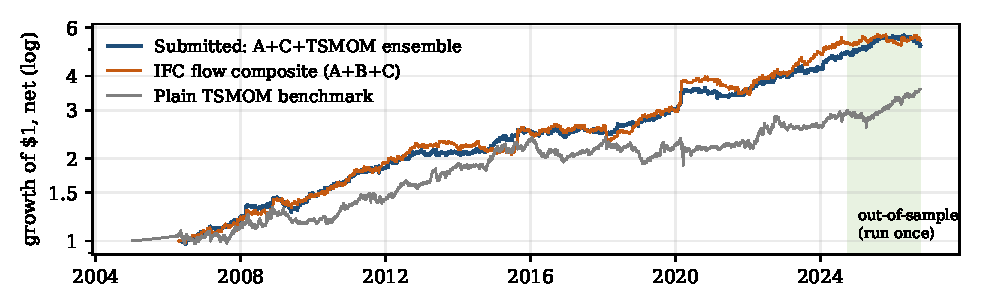
\includegraphics[width=\linewidth]{fig_equity.pdf}
\vspace{-14pt}
\caption{Growth of \$1, net of costs. The shaded period was evaluated once, after the selection was committed.}
\vspace{-8pt}
\end{figure}

\begin{table}[h]\centering\small
\caption{Every pre-registered stream and replication: net Sharpe ratio. Futures in-sample starts 2010-06.}
\vspace{-2pt}\setlength{\tabcolsep}{4.5pt}
\begin{tabular}{@{}lccc@{\hspace{10pt}}|@{\hspace{8pt}}lcc@{}}
\toprule
ETF streams & IS & OOS & OOS 2x & Composites / futures & IS & OOS\\
\midrule
A rebalancing pressure & \isA & \oosA & \oostwoA & IFC flow composite A+B+C & \IFCsr & \IFCoos\\
B dash for cash & \isB & \oosB & \oostwoB & IFC-F on ES/ZN (Databento) & \IFCFsr & \IFCFoos\\
C Treasury month end & \isC & \oosC & \oostwoC & PCT-F, 20 futures & \PCTFsr & \PCTFoos\\
D FX hedge (exploratory) & \isD & \oosD & \oostwoD & TSMOM-F, 20 futures & \TSMOMFsr & \TSMOMFoos\\
E auction cycle (exploratory) & \isE & \oosE & \oostwoE & ID-conditioned trend-F & \IDFsr & \IDFoos\\
PCT (path-geometry trend) & \isP & \oosP & \oostwoP & & & \\
TSMOM benchmark & \isT & \oosT & \oostwoT & & & \\
ID-conditioned trend & \isI & \oosI & \oostwoI & & & \\
\bottomrule
\end{tabular}
\vspace{-6pt}
\end{table}

\textbf{In-sample evidence.} Sharpe by sub-period: \suba{} (2006--08), \subb{} (2009--12), \subc{} (2013--16), \subd{} (2017--20), \sube{} (2021--24); best year \bestyr{} of P\&L; positive in 2008 and 2022; 90\% block-bootstrap interval [\bootlo, \boothi]. Factor loadings are small (market \ISmktbeta, momentum \ISmombeta, Treasury duration \ISbondbeta). One-step neighbours have median Sharpe \nbrmed; the median of all \nconfigs{} configurations is \cfgmedian, so diversification, not a lucky configuration, drives the result (PBO \PBO). With all \ntrials{} trials the expected maximum Sharpe under no skill is \SRzero{} and the Deflated Sharpe is \DSR; the trials are so correlated that their effective number is \neff{} (eigenvalue participation), giving \DSReff. The flow composite (A+B+C) has in-sample alpha \IFCalpha{} ($t=\IFCalphat$), but timing matters: shifting every window one day earlier/later gives \IFCshiftE/\IFCshiftL, and one extra day of delay gives \IFCdelay.\\
\textbf{What failed in-sample.} The settlement natural experiment: the old fixed T+3 windows did as well as the settlement-aware ones (\Bfixed{} vs \isB), so B2 is rejected. Issuance sizing added nothing to C (\Cq{} without it). PCT did \emph{not} beat plain TSMOM (\isP{} vs \isT), on ETFs or futures (\PCTFsr{} vs \TSMOMFsr): its kill condition triggered. The information-discreteness variant (Da, Gurun \& Warachka 2014) did improve trend on both universes (\isI, \IDFsr). FX hedge flows and the auction cycle failed, as the decay literature predicted for the latter.\\
\textbf{Out-of-sample.} Gross of costs the strategy still earned a Sharpe of \OOSgross; costs on \OOSto$\times$ annual turnover took it to \OOSsr. Contributions: A \contA, C \contC, trend \contT{} a year. Raw effects (Figure 2, no strategy code): IEF earned \CoosIEF{} bp/day over $[T{-}2,T]$ versus \CoosOther{} on other days (in-sample \CisIEF{} vs \CisOther); the drift-signed bond-minus-stock spread over $[T{-}4,T]$ fell from \AisSpr{} to \AoosSpr{} bp/day. The rebalancing paper became public in March 2025, inside the window, consistent with post-publication decay (McLean \& Pontiff 2016). The strategy's in-sample two-year rolling Sharpe had median \rollmed, 5th percentile \rollpfive{} and minimum \rollmin: the out-of-sample result is unusually poor, not ordinary noise. PCT, rejected in-sample, was the best out-of-sample stream (\oosP); we do not switch to it, since that would be selection on the test set.

\begin{figure}[h]\centering
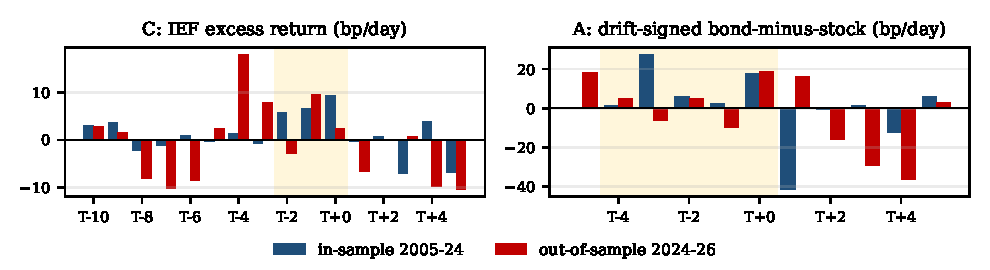
\includegraphics[width=\linewidth]{fig_event.pdf}
\vspace{-14pt}
\caption{Mean daily excess return by trading day relative to month end $T$; shaded: traded window. Right panel signs the bond-minus-stock spread by the 60/40 drift observed at $T{-}6$; the post-turn reversal is what temporary price pressure predicts.}
\vspace{-6pt}
\end{figure}

\sect{6. Risk management}
\textbf{Limits.} Gross exposure $\le 4\times$ and $\le 3\times$ per ETF (binding on 12\% of days, the month-end windows); average gross \grossmean$\times$. Each stream is vol-scaled at entry; the portfolio targets 8\% volatility from a lagged 63-day EWMA, so exposure falls automatically after volatility spikes. The cap bounds single-window losses: a 3-day 4$\times$ IEF window loses about 2.8\% per one-sigma rate move (5.7\% at two sigma); the worst in-sample month was \ISworst. \textbf{Pre-set de-risking.} The pre-registered drawdown brake (halve exposure 10\% below peak) never triggered in-sample at 1x costs; we would run it live, plus a stop on each mechanism if its rolling 24-month raw effect (Figure 2) turns negative, which the out-of-sample data would have tripped for A. \textbf{Factor and regime exposure.} Market and momentum betas are near zero; the duration beta (\ISbondbeta) comes from sleeve C and is the main macro risk (it is a long-duration bet three days a month). The strategy made money in 2008, 2020 and 2022 (positive stock-bond correlation). Daily skew is positive (\ISskew): the contrarian legs are not short volatility. \textbf{Event risk.} CPI, payrolls or FOMC inside a month-end window can dominate a 3--5 day position; live, we would skip or halve windows containing a scheduled top-tier release.

\sect{7. Liquidity and capacity}
Square-root impact, cost $=$ fixed $+\ \sigma_{\text{daily}}\sqrt{\text{trade}/\text{ADV}}$, using each instrument's trailing 63-day median dollar volume and the strategy's actual trades. Net Sharpe by assets under management:
\begin{center}\small\vspace{-4pt}
\begin{tabular}{@{}lccccc@{}}\toprule
AUM & \$0 (fixed costs only) & \$1M & \$10M & \$100M & \$1B\\\midrule
ETF ensemble (2019--24 liquidity) & \capEZero & \capEOne & \capETen & \capEHund & \capEBil\\
Futures, IFC-F (2010--24) & \capFZero & \capFOne & \capFTen & \capFHund & \capFBil\\\bottomrule
\end{tabular}\vspace{-4pt}\end{center}
The ETF version concentrates up to 4$\times$ NAV of IEF (secondary volume about \$0.5bn a day) into month-end windows, so it is a 20-year proof of the effect, not a vehicle: its edge halves near \$1--2M. This is conservative, since ETF screen volume understates liquidity reachable through creation/redemption against the Treasury cash market. ZN and ES trade \$50--300bn a day, so the futures implementation keeps half its edge near \$1bn. Turnover is high (\ISto$\times$/yr), which is why costs, not signal, decided the out-of-sample result.

\sect{8. Limitations and next steps}
The out-of-sample window holds only 24 month-ends, so a two-year Sharpe has a standard error near 0.7; still, the result sits at the bottom of the in-sample distribution and both mechanisms weakened, so we read it as decay, not bad luck. Daily bars cannot time the 4\,pm close or intraday flow; ETF adjusted prices are revised retroactively (we snapshot them); the variant count, though fully logged, is large. Next: (1) trade only the futures version with market-on-close execution and monitor each mechanism's raw effect live; (2) intraday Databento data to locate when month-end flows now hit (the OOS profile suggests earlier and after the turn); (3) treat the information-discreteness trend result, which replicated across ETF and futures universes, as a new pre-registered hypothesis rather than a post-hoc fix.

\vspace{-2pt}
\begin{small}
\sect{References}
Bailey, D., L\'opez de Prado, M. (2014), The Deflated Sharpe Ratio, \emph{J.\ Portfolio Management}.
Bailey, D., Borwein, J., L\'opez de Prado, M., Zhu, Q. (2017), The Probability of Backtest Overfitting, \emph{J.\ Computational Finance}.
Da, Z., Gurun, U., Warachka, M. (2014), Frog in the Pan, \emph{Review of Financial Studies}.
Etula, E., Rinne, K., Suominen, M., Vaittinen, L. (2020), Dash for Cash, \emph{Review of Financial Studies}.
Hartley, J., Schwarz, K. (2019), Predictable End-of-Month Treasury Returns, working paper.
Harvey, C., Mazzoleni, M., Melone, A. (2025), The Unintended Consequences of Rebalancing, NBER WP 33554.
Harvey, C., Liu, Y., Zhu, H. (2016), \ldots and the Cross-Section of Expected Returns, \emph{RFS}.
Ledoit, O., Wolf, M. (2004), A well-conditioned estimator for large covariance matrices, \emph{J.\ Multivariate Analysis}.
Lou, D., Yan, H., Zhang, J. (2013), Anticipated and Repeated Shocks in Liquid Markets, \emph{RFS}.
McLean, R., Pontiff, J. (2016), Does Academic Research Destroy Stock Return Predictability?, \emph{J.\ Finance}.
Melvin, M., Prins, J. (2015), Equity Hedging and Exchange Rates at the London 4 p.m.\ Fix, \emph{J.\ Financial Markets}.
Moskowitz, T., Ooi, Y., Pedersen, L. (2012), Time Series Momentum, \emph{J.\ Financial Economics}.
Almgren, R., Thum, C., Hauptmann, E., Li, H. (2005), Direct Estimation of Equity Market Impact, \emph{Risk}.
Data: Yahoo Finance; FRED; Kenneth R.\ French Data Library; U.S.\ Treasury Fiscal Data; Databento (GLBX.MDP3).
Prior work extended: github.com/minh-stakc/physics-quant-research. Code was written with AI assistance; all results reproduce from the repository with \texttt{run\_all.py}.
\end{small}
\end{document}
